\section{Schutzelemente}
\label{sec:Schutz}
%Was für Schutzelemente gibt es?
%Wie kann die Schaltung geschützt werden?
Um eine Schaltung vor EMV-Störgrössen zu schützen, gibt es verschiedene Schutzelement. Nachfolgend werden Schutzelemente für Burst und Surge, die Testarten welche im vorhergehenden Kapitel ausgewählt wurden, vorgestellt.\\[0.25cm]
Wie im vorhergehenden Kapitel erwähnt, ist der Burst eine HF-Störung, welche Leitungsgebunden ist. Der hohne Frequenz kann mit einem Entkopplungskondensator oder einem Tiefpassfilter entgegnet werden.\\[0.25cm]
Der Surge gibt Stossspannungen ab, welche einen zu hohen Spannungspegel und eine erhöhte Frequenz aufweisen. Der erhöhte Spannungspegel kann mit verschiedenen Schutzelementen entgegnet werden.
\vspace*{-0.5cm} 
\subparagraph*{Varistor:} Ein Varistor ist ein Widerstand, welcher einen Leitwert besitzt der sich mit steigender Spannung erhöht. Die Erhöhung des Leitwertes erfolgt über den Aufbau eines E-Feldes, das die Sperrschichten überwindet. Ab einer bestimmten Spannung wird der Varistor stark leitend und verhindert so einen weiteren Spannungsanstieg.
\vspace*{-0.5cm} 
\subparagraph*{Thermistor:} Der Thermistor ist ein temperaturabhängiger Widerstand. Es gibt PTC (Kaltleiter), welche bei einem hohen Strom, was einen hohen Temperaturanstieg zur Folge hat, hochohmig werden und so den Strom verringern. Ebenso gibt es NTC (Heissleiter), welche bei einem hohen Strom niederohmig werden und somit mehr Strom durchlassen. Thermistoren werden auch rückstellbare Sicherung genannt, da diese ihren ursprünglichen Widerstandswert wiedereinnehmen, sobald sich der Strom (und somit auch die Temperatur) wieder gelegt hat.
\vspace*{-0.5cm} 
\subparagraph*{Gasableiter:} Ähnlich wie die vorhergehenden Schutzelemente wird auch der Gasableiter bei Überspannung stark leitend. Dieser ist jedoch nicht geeignet für Gleichstrom, da im Nulldurchgang der Strom gelöscht wird.
\vspace*{-0.5cm} 
\subparagraph*{Suppresserdiode:}Auch TVS-Diode genannt, leiten den Spannungsüberschuss ab. Sie verfügen über ein schnelles Reaktionsvermögen und besitzen jedoch eine Durchbruchspannungsstreuung.\\[0.25cm]
Die Schaltung besitzt bereits eine Tiefpassfilterung. Trotzdem wird noch ein Entkopplungskondensator von 100nF hinzugefügt. Um dem Surge zu entgegnen wird eine Suppresserdiode (P6KE6.8) verwendet, welche eine Sperrspannung von 5.5 Volt besitzt. Diese zwei Elemente werden parallel vor dem Shunt hinzugefügt, wie in Abbildung \ref{fig:Schema2} zu sehen ist.\\[0.25cm]
\begin{minipage}[b][4.75cm][t]{1\textwidth}
\centering
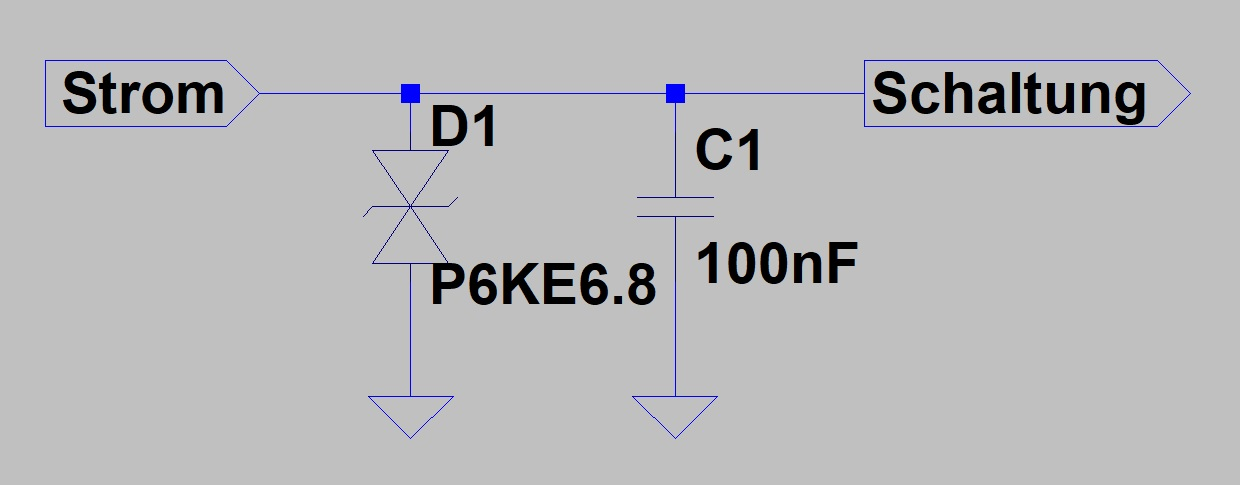
\includegraphics[angle=0,width=0.6\textwidth]{graphics/Schema2.jpg}
\captionof{figure}{Ergänzung des Schemas.}
\label{fig:Schema2}
\end{minipage}
Abbildung \ref{fig:Schema2} zeigt den ergänzten Teil des Schemas, welches in Abbildung \ref{fig:SchaltungDraw} zu sehen ist. Abbildung \ref{fig:Schaltung1} zeigt bereits die gesamte Schaltung mit den Schutzelementen (5). Die geschützte Schaltung soll nun getestet werden, dafür wird im nächsten Kapitel auf den Testaufbau eingegangen.

